% Config
\documentclass{beamer}
\usepackage[utf8]{inputenc}

% Packages
\usepackage{multicol}
\usepackage[francais]{babel}
\usepackage{amsfonts, amsthm, amssymb, amsmath}
\usepackage{xcolor}
\usepackage{mathtools}
\usepackage{ninecolors}
\usepackage{physics}
\usepackage{hyperref}
\usepackage{adjustbox}
\usepackage{listings}

\hypersetup{colorlinks=true, linkcolor=black, urlcolor=black}

\title{TP5 Thermodynamique}
\author{BERREDO DE LA COLINA Lucas\\ MARTIN Lola}
\date{}

\usetheme[nofirafonts]{focus}

\lstset{frame=tb,
  language=Python,
  aboveskip=3mm,
  belowskip=3mm,
  showstringspaces=false,
  columns=flexible,
  basicstyle={\small\ttfamily},
  numbers=none,
  numberstyle=\tiny\color{gray},
  keywordstyle=\color{blue},
  commentstyle=\color{darkgreen},
  stringstyle=\color{mauve},
  breaklines=true,
  breakatwhitespace=true,
  tabsize=4
}

% Commands
\newcommand{\newlines}{\newline\newline}



% Document
\begin{document}




\begin{frame}

\Huge{TP5 Thermodynamique}

\Large{Partie 1: Rayonnement}
\\[2em]
\large{BERREDO DE LA COLINA Lucas\\ MARTIN Lola}

\end{frame}





\begin{frame}
\frametitle{Rappel théorique}

\begin{itemize}
	\item{Corps noir / corps gris}
	\item{Radiation dans le vide}

\end{itemize}

\end{frame}





\begin{frame}
\frametitle{Explication théorique}

\begin{itemize}
	\item{Analogue électrocinétique}
	\item{Résolution exacte}
	\item{Résolution approchée}
	
\end{itemize}

\end{frame}





\begin{frame}
\frametitle{Dispositif expérimental}

\begin{itemize}
	\item{Deux échantillons (gris, noir)\newline}
	\item{Deux chambres:\newline
	\begin{itemize}
		\item{Four ($200^{\circ}C$)\newline}
		\item{Refroidessement à l'eau\newline}
	\end{itemize}}
	\item{Elles peuvent être mises sous vide\newline}
	\item{Mesures de temperature analogiques (100 points, 15 min)}
\end{itemize}
\end{frame}





\begin{frame}
\frametitle{Experiences}

\begin{enumerate}
	\item{{\color{gray7}Corps gris}{\color{gray4}, {\color{red}chauffage}, vide}\newline}
	\item{{\color{gray7}Corps gris}{\color{gray4}, {\color{blue5}refroidissement}, vide}\newline}
	\item{{\color{gray7}Corps gris}{\color{gray4}, {\color{red}chauffage}, sans vide}\newline}
	\item{{\color{gray7}Corps gris}{\color{gray4}, {\color{blue5}refroidissement}, sans vide}\newline}
	\item{{\color{black}Corps noir}{\color{gray4}, {\color{red}chauffage}, vide}\newline}
	\item{{\color{black}Corps noir}{\color{gray4}, {\color{red}chauffage}, sans vide}\newline}

\end{enumerate}
\end{frame}





\begin{frame}
\frametitle{Organisation des données}

\centering
\begin{minipage}{0.48\textwidth}
    \centering
    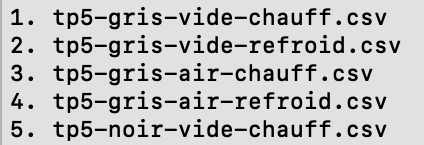
\includegraphics[width=\linewidth]{Fig/ls-csv.png}
\end{minipage}
\hfill
\begin{minipage}{0.48\textwidth}
    \centering
    \adjustbox{valign=c}{
        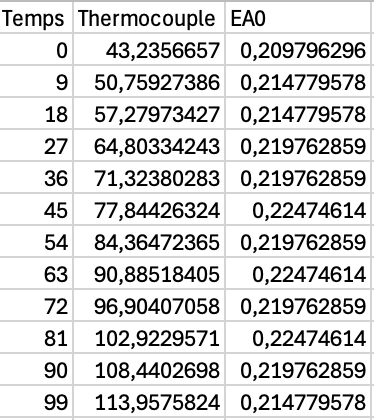
\includegraphics[width=\linewidth]{Fig/example-csv.png}}
\end{minipage}
\end{frame}





\begin{frame}
\frametitle{Approximation graphique 1er ordre}

Il ne faut que vérifier les valeur initiales, finales et approcher $\tau$ de façon qu'on trouve des courbes proches

\begin{figure}
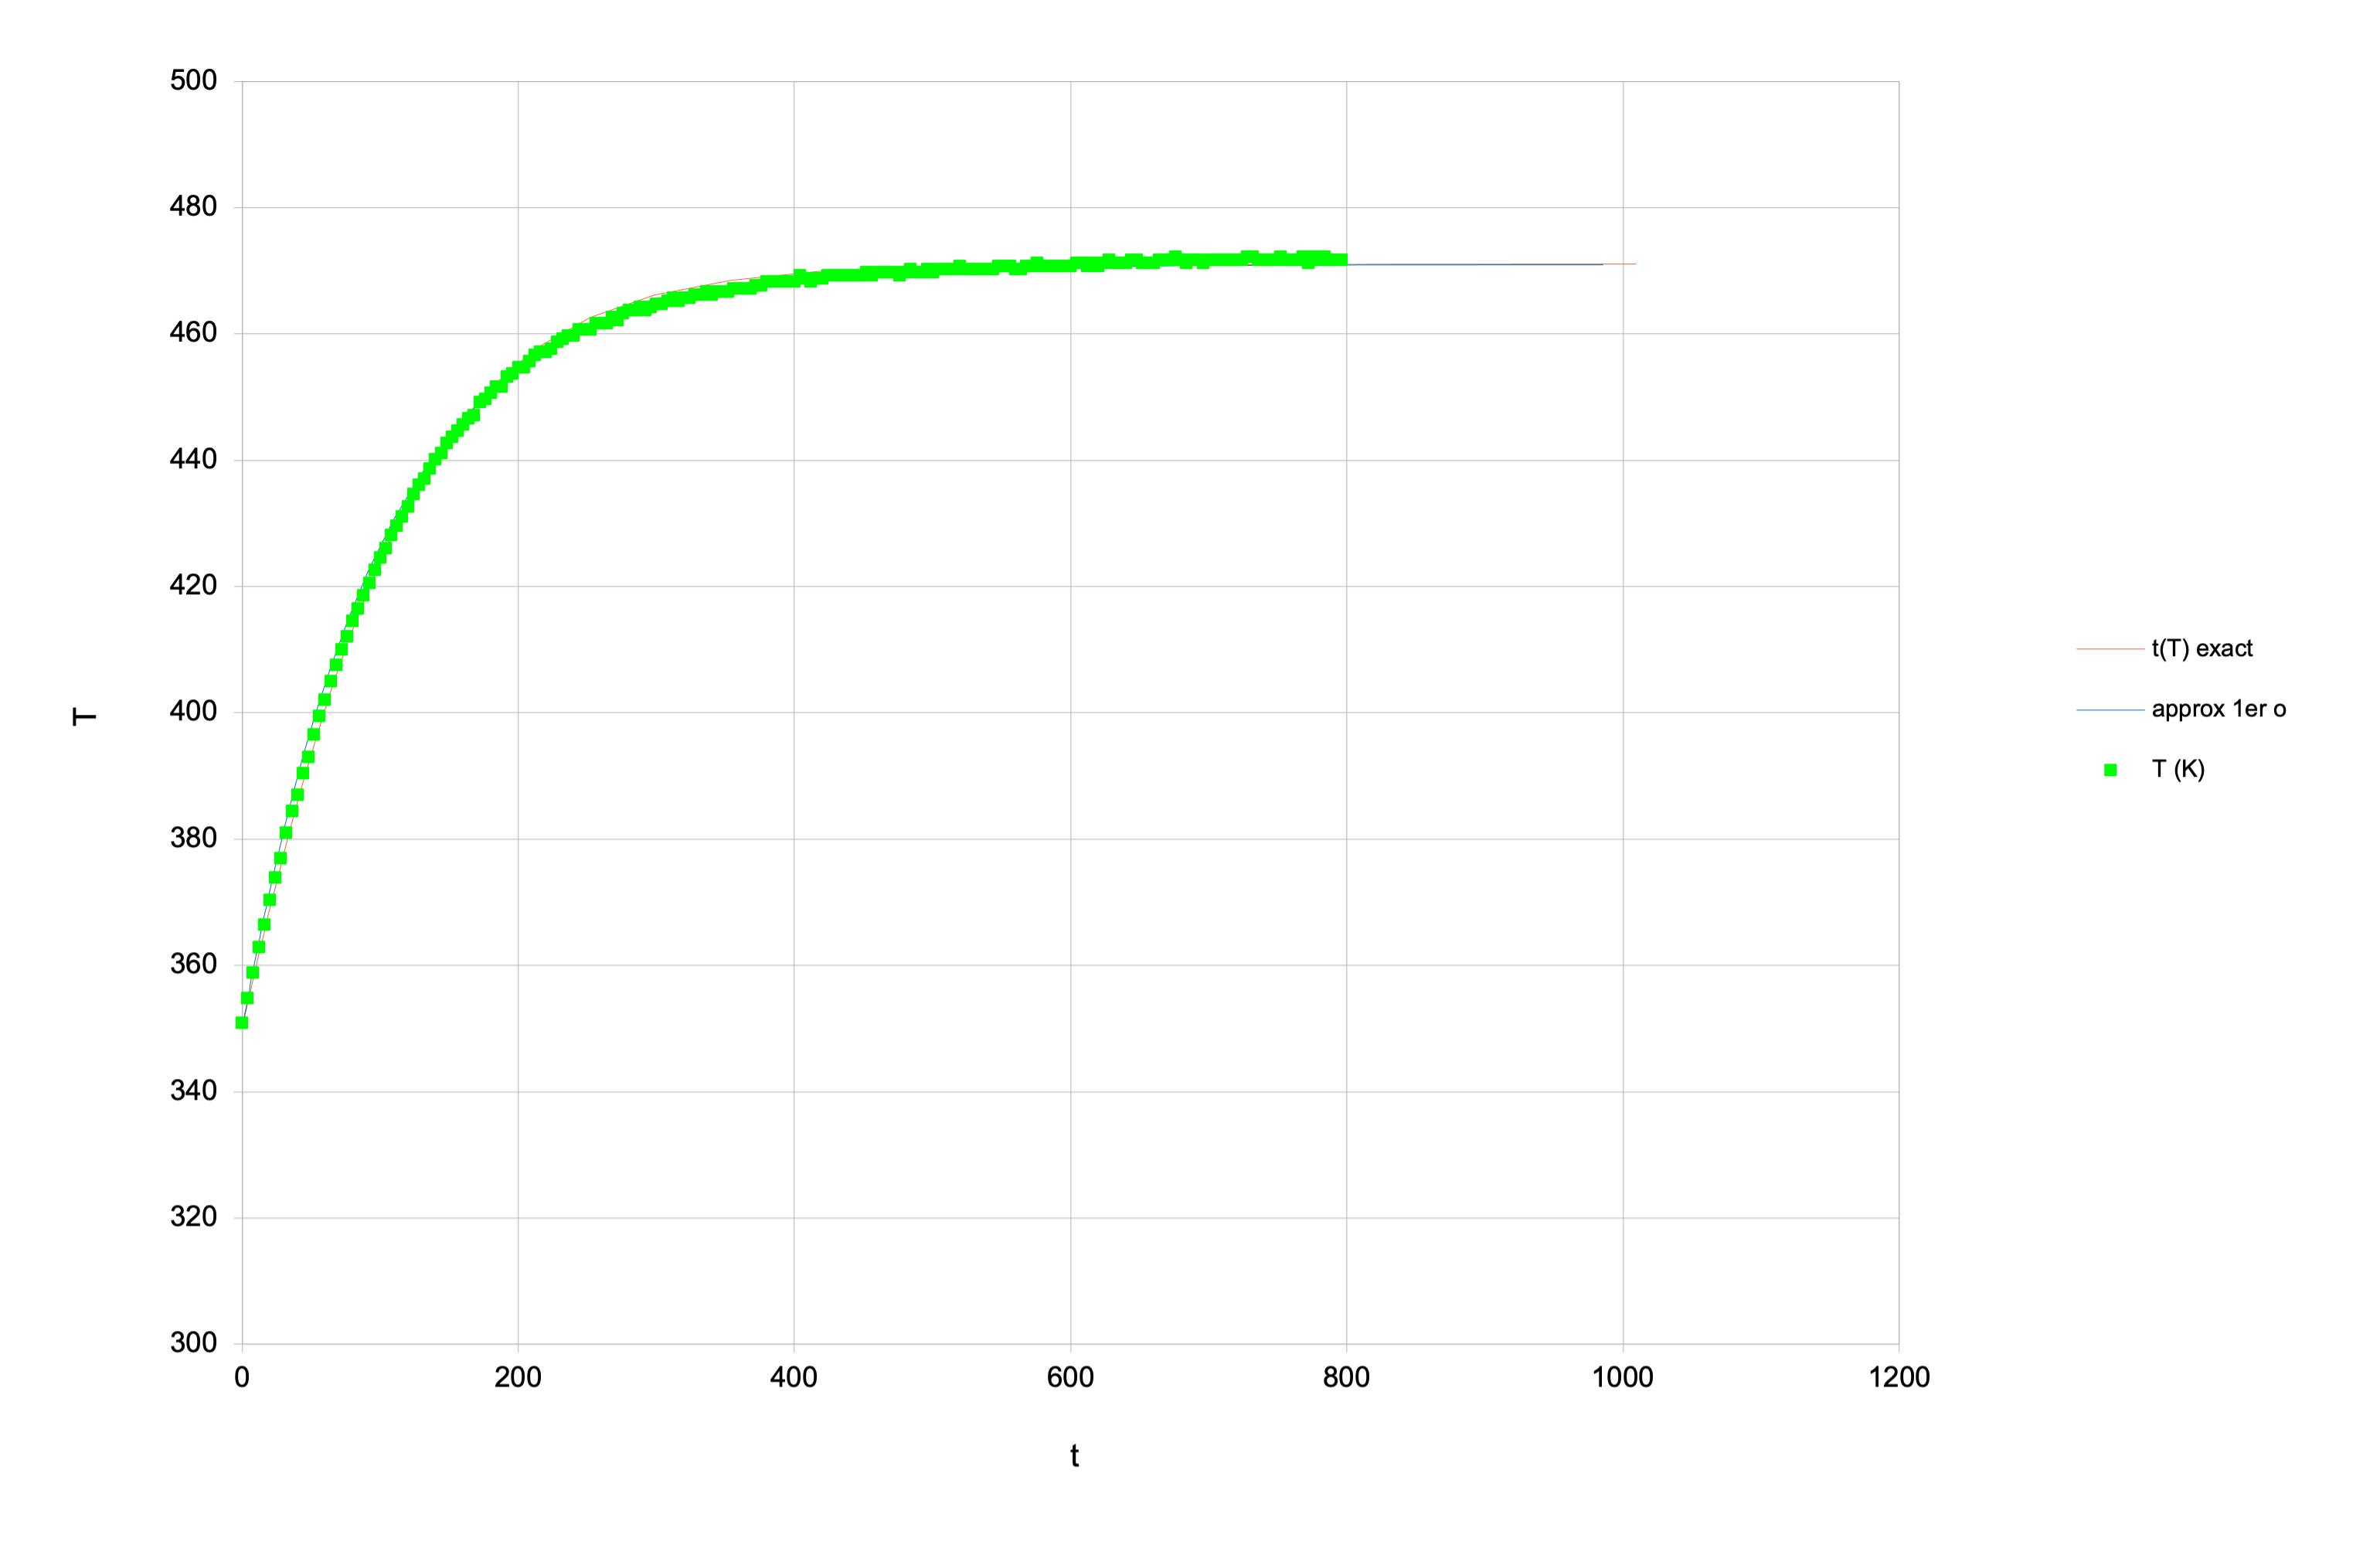
\includegraphics[width=0.75\textwidth]{Fig/t1-100-t2-82.png}
\caption{Example representation graphique: Vert: points experimentaux, Bleu: courbe théorique}
\end{figure}

\end{frame}





\begin{frame}
\frametitle{Approximation graphique 1er ordre}

Nous obtenons les prochains valeurs:
\begin{enumerate}
	\item{{\color{gray7}Corps gris}{\color{gray4}, {\color{red}chauffage}, vide} \hfill $\tau = $\hspace{4em} \newline}
	\item{{\color{gray7}Corps gris}{\color{gray4}, {\color{blue5}refroidissement}, vide} \hfill $\tau = $\hspace{4em} \newline}
	\item{{\color{gray7}Corps gris}{\color{gray4}, {\color{red}chauffage}, sans vide} \hfill $\tau = $\hspace{4em} \newline}
	\item{{\color{gray7}Corps gris}{\color{gray4}, {\color{blue5}refroidissement}, sans vide} \hfill $\tau = $\hspace{4em} \newline}
	\item{{\color{black}Corps noir}{\color{gray4}, {\color{red}chauffage}, vide} \hfill $\tau = $\hspace{4em} \newline}
	\item{{\color{black}Corps noir}{\color{gray4}, {\color{red}chauffage}, sans vide}\hfill $\tau = $\hspace{4em} \newline}
\end{enumerate}
\end{frame}





\begin{enumerate}
\frametitle{Approximation graphique 2ème ordre}
\begin{enumerate}
	\item{{\color{gray7}Corps gris}{\color{gray4}, {\color{red}chauffage}, vide} \hfill $\tau = $\hspace{4em} \newline}
	\item{{\color{gray7}Corps gris}{\color{gray4}, {\color{blue5}refroidissement}, vide} \hfill $\tau = $\hspace{4em} \newline}
	\item{{\color{gray7}Corps gris}{\color{gray4}, {\color{red}chauffage}, sans vide} \hfill $\tau = $\hspace{4em} \newline}
	\item{{\color{gray7}Corps gris}{\color{gray4}, {\color{blue5}refroidissement}, sans vide} \hfill $\tau = $\hspace{4em} \newline}
	\item{{\color{black}Corps noir}{\color{gray4}, {\color{red}chauffage}, vide} \hfill $\tau = $\hspace{4em} \newline}
	\item{{\color{black}Corps noir}{\color{gray4}, {\color{red}chauffage}, sans vide}\hfill $\tau = $\hspace{4em} \newline}
\end{enumerate}

\end{enumerate}





\begin{frame}
\frametitle{Approximation numérique avec Python}
Comme nous avons la résolution pour $\tau$, nous pouvons donner ça vers un $\texttt{curve\_fit}$ dans Python.

\begin{figure}
\includegraphics[width=\textwidth]{Fig/Python_Refroid.png}
\caption{Exemple refroidissement. Il y a aussi un fichier pour chauffement.}
\end{figure}

\end{frame}






\begin{frame}
\frametitle{Comparaison des résultats}

\end{frame}





\begin{frame}
\frametitle{Explication des résultats}

\end{frame}





\begin{frame}
\frametitle{Approximation numérique avec Python}
Résultats:
\begin{enumerate}
	\item{{\color{gray7}Corps gris}{\color{gray4}, {\color{red}chauffage}, vide} \hfill $\tau = 96.0399...$\hspace{4em} \newline}
	\item{{\color{gray7}Corps gris}{\color{gray4}, {\color{blue5}refroidissement}, vide} \hfill $\tau = 86.1429...$\hspace{4em} \newline}
	\item{{\color{gray7}Corps gris}{\color{gray4}, {\color{red}chauffage}, sans vide} \hfill $\tau = 99.2634...$\hspace{4em} \newline}
	\item{{\color{gray7}Corps gris}{\color{gray4}, {\color{blue5}refroidissement}, sans vide} \hfill $\tau = 84.5618...$\hspace{4em} \newline}
	\item{{\color{black}Corps noir}{\color{gray4}, {\color{red}chauffage}, vide} \hfill $\tau = 111.8591...$\hspace{4em} \newline}
	\item{{\color{black}Corps noir}{\color{gray4}, {\color{red}chauffage}, sans vide}\hfill $\tau = 90.5110...$\hspace{4em} \newline}
\end{enumerate}
\end{frame}





\begin{frame}

\Huge{TP5 Thermodynamique}

\Large{Partie 2: Loi de Stefan}
\\[2em]
\large{BERREDO DE LA COLINA Lucas\\ MARTIN Lola}

\end{frame}





\begin{frame}
\frametitle{Avertissement}
Bien que nous ayons travaillé avec l'équipement et observé des résultats avec {\color{red} Mme Nom}, nous n'avons pas enregistré de résultats numériques.
\end{frame}





\begin{frame}
\frametitle{Rappel théorique}

\begin{itemize}
	\item{Deduction Loi Stefan}

\end{itemize}

\end{frame}





\begin{frame}
\frametitle{Dispositif experimental}

\begin{itemize}
	\item{Explication dispositif}
	
\end{itemize}	
	
\end{frame}





\begin{frame}
\frametitle{Approximation des résultats}

\begin{itemize}
	\item{Rappel: on n'a pas les résultats, mais on peut approximer}
	\item{Simulation des données}
	\item{Explication du valeur}
	
\end{itemize}
\end{frame}


\end{document}